\documentclass[10pt,a4paper]{article}

\usepackage[margin=2cm]{geometry}
\usepackage[T1]{fontenc}
\usepackage{lmodern}
\usepackage{amsmath,amssymb}
\usepackage{booktabs,tabularx,array}
\usepackage{graphicx}
\usepackage[font=normalsize,labelfont=bf]{caption}
\usepackage{xcolor}
\usepackage[hidelinks]{hyperref}

\definecolor{navy}{HTML}{244A6B}
\definecolor{lightblue}{HTML}{EAF2F8}
\definecolor{rulegray}{HTML}{8A98A5}

\setlength{\parindent}{0pt}
\setlength{\parskip}{3.4pt plus 1pt minus 1pt}
\setlength{\tabcolsep}{5pt}
\renewcommand{\arraystretch}{1.10}
\captionsetup{skip=3pt}
\newcolumntype{Y}{>{\raggedright\arraybackslash}X}
\newcolumntype{R}{>{\raggedleft\arraybackslash}p{1.65cm}}
\newcommand{\metric}[1]{\textsc{#1}}
\newcommand{\code}[1]{\texttt{#1}}

\begin{document}

\begin{titlepage}
\thispagestyle{empty}
\centering
\vspace*{1.0cm}

\includegraphics[width=0.42\textwidth]{report_assets/nus_logo.jpg}\par
\vspace{2.2cm}
{\Large\bfseries DSA5101\par}
\vspace{0.35cm}
{\large\bfseries Introduction to Big Data for Industry\par}
\vspace{2.4cm}
{\LARGE\bfseries Friendship Communities and Music Recommendation:\par}
\vspace{0.25cm}
{\Large A Comparative Study Using Last.fm Data\par}
\vfill
{\large Huang Wanlu A0237821E\par}
\vspace{1.0cm}
\end{titlepage}

{\LARGE\bfseries\color{navy} Friendship Communities and Music Recommendation:\\[-1pt] A Comparative Study Using Last.fm Data}\par
\vspace{5pt}
\hrule height 0.8pt
\vspace{6pt}

\begin{table}[h]
\centering
\caption*{Executive summary}
\begin{tabularx}{\textwidth}{>{\bfseries\raggedright\arraybackslash}p{2.75cm}Y}
\toprule
Project title & \emph{Friendship Communities and Music Recommendation: A Comparative Study Using Last.fm Data}. \\
Dataset and source & HetRec 2011 Last.fm 2K, released with the HetRec 2011 workshop \cite{cantador2011}. The working data contain 92,834 positive user-artist pairs from 1,892 users, 17,632 artists, and 12,717 undirected friendship links. \\
Research question & Do friendship-graph communities improve artist recommendation beyond implicit alternating least squares (ALS), especially for users with sparse observed histories? \\
Algorithm classes & Matrix factorization (implicit ALS, DSA5101 Lecture 5) and community detection (Louvain, DSA5101 Lecture 7). Global popularity is used as a baseline, and the two signals are combined in a normalized hybrid. \\
Evaluation design & Macro binary-relevance NDCG@10 on a shared fit-only candidate universe, with validation-based model selection, a held-out test set, and a paired user bootstrap for the primary hybrid-versus-ALS comparison. \\
Key finding & The hybrid achieved NDCG@10 of 0.241904 versus 0.239324 for ALS. The paired difference was $+0.002579$, with a 95\% bootstrap interval of $[-0.000008,0.005026]$; therefore, the planned evidence for improvement over ALS was not established. \\
\bottomrule
\end{tabularx}
\end{table}

\section{Research question and dataset}

The question is whether communities detected in a friendship graph add useful ranking information beyond a listening-history model, with a planned focus on sparse-history users. The study considers three related questions: listening similarity within communities, hybrid versus ALS recommendation performance, and sparse-history subgroup analysis. The hybrid-versus-ALS comparison is the primary inferential analysis.

The study uses HetRec 2011 Last.fm 2K, released with the HetRec 2011 workshop \cite{cantador2011}. The archive contains aggregate listening counts, not events: each of the 92,834 rows is a distinct positive user-artist pair. It covers 1,892 users and 17,632 artists. Reciprocal friendship records were canonicalized to 12,717 simple undirected edges. Tags were not used. The source is a historical convenience sample; it is not representative of all Last.fm users.

There are no listening-event timestamps. The holdout therefore measures recovery of randomly withheld observed pairs, not future recommendation. Friendship, community membership, and listening may share unmeasured causes. No result identifies social influence, a causal friendship effect, or deployment performance.

\section{Data preparation}

The source files were checked for readable ZIP contents, expected schemas and keys, positive weights, valid catalog references, and reciprocal friendships before analysis. The indivisible unit was a user-artist pair with its original count.

Within each user, a fixed ordering based on seed 5101, user ID, and artist ID was used, with artist ID as the tie-break. Users with at least seven pairs received a largest-remainder 70/15/15 allocation across train, validation, and test. The 16 lower-history users contributed all 38 pairs only to fitting and never to metrics. This conserved all 92,834 pairs:

\begin{table}[h]
\centering
\begin{tabular}{lrr}
\toprule
Partition & Pairs & Users \\
\midrule
Train & 64,958 & 1,876 \\
Validation & 14,842 & 1,876 \\
Test & 12,996 & 1,876 \\
Fit-only, low history & 38 & 16 \\
\bottomrule
\end{tabular}
\end{table}

For a phase, the primary universe was the set of artists in that phase's fitting data. A user's candidates were this universe minus their fitting artists, identically for every method. Relevance was the held-out artist set intersected with those candidates. Thus, fit-absent held-out artists were recorded as cold and excluded from the primary metric rather than treated as retrievable misses. Validation fitting used train plus low-history fit-only rows; final fitting added validation rows. Test data did not influence fitting or selection.

Sparse status was defined before model selection from split-training distinct-artist counts. The nearest-rank first quartile was 35 and ties were included. All 1,876 evaluation-eligible users were at or below that cutoff because source histories are capped and 1,829 users have exactly 35 training artists. This left no non-sparse comparison group, and the definition was not revised after observing the distribution.

\section{Methods and how they connect}

All components use fit-only data and feed a common top-10 ranking and evaluation layer. The two main course connections are \textbf{Matrix Factorization (DSA5101 Lecture 5)}, implemented through implicit ALS, and \textbf{Community Detection (DSA5101 Lecture 7)}, implemented through Louvain clustering of the friendship graph. Listening count $w_{ui}$ becomes activity $a_{ui}=\log(1+w_{ui})$. Global popularity scores item $i$ by $\sum_u a_{ui}$ and provides both a baseline and the global distribution used for community shrinkage.

Louvain modularity optimization \cite{blondel2008} was applied once to the static undirected friendship graph with seed 5101, sorted input, and deterministic label canonicalization. It found 32 communities (modularity 0.4526). A community profile used
\[
 P(i\mid c)=\frac{s_{ci}+\beta q_i}{s_c+\beta},\qquad
 q_i=\frac{\sum_u a_{ui}}{\sum_{u,j}a_{uj}},
\]
where $s_{ci}$ and $s_c$ are community fit-activity totals. This connects topology to recommendation only through fit-derived artist profiles; no held-out listening value enters community detection or profiling.

\begin{figure}[h]
\centering
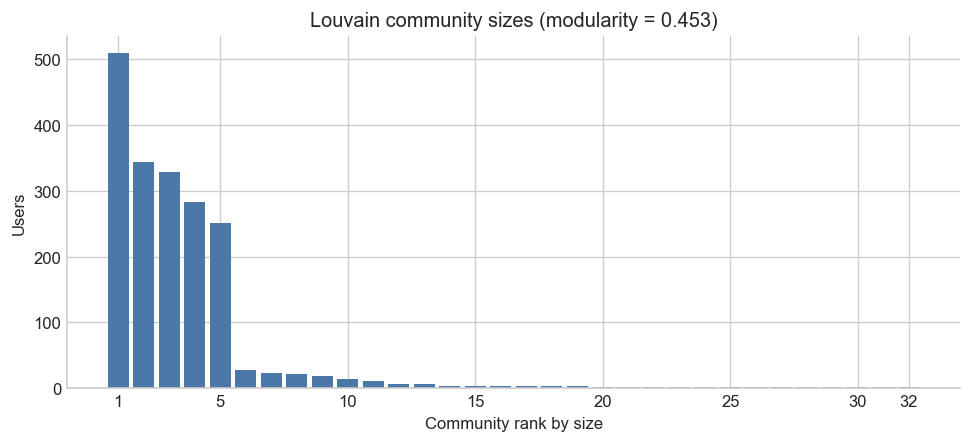
\includegraphics[width=0.88\textwidth]{report_assets/community_sizes.png}
\caption{Louvain community sizes from the executed notebook. Bars are ordered by size; all 1,892 users have one assignment. The marked imbalance motivates shrinkage of community artist frequencies toward the global activity distribution.}
\label{fig:communities}
\end{figure}

Implicit ALS follows the confidence-weighted formulation for implicit feedback \cite{hu2008}: preference is $p_{ui}=1$ for observed pairs and 0 otherwise, with confidence $c_{ui}=1+\alpha\log(1+w_{ui})$. The objective is
\[
 \sum_{u,i}c_{ui}(p_{ui}-x_u^\top y_i)^2+\gamma\left(\sum_u\lVert x_u\rVert^2+\sum_i\lVert y_i\rVert^2\right).
\]
The hybrid z-normalizes finite ALS scores and finite $\log P(i\mid c)$ scores over each user's shared candidate set using the population standard deviation, then computes $\lambda z_{\rm ALS}+(1-\lambda)z_{\rm community}$. This normalization makes unlike score scales combinable; candidates missing either required component remain missing rather than being imputed.

Validation alone selected hyperparameters by macro NDCG@10. The candidate grid contained 8 ALS settings (factors 32/64, regularization 0.01/0.10, $\alpha$ 1/10), 3 community values ($\beta=10,100,1000$), and 9 hybrid pairs ($\beta=10,100,1000$; $\lambda=0.25,0.50,0.75$). Selected values were ALS factors 32, regularization 0.10, $\alpha=1$; community $\beta=1000$; and hybrid $\beta=100$, $\lambda=0.25$. ALS used 20 iterations and seed 5101. No parameter changed after test inspection.

Ranking used ascending artist ID to break score ties. Primary NDCG@10 used binary relevance and the standard logarithmic discount \cite{jarvelin2002}; Recall@10 and catalog coverage@10 were secondary. Macro averages give every metric-eligible user equal weight.

\section{Evaluation and results}

The final primary candidate universe contained 16,057 fit-observed artists. Of 1,876 raw evaluation-eligible users, 1,872 had at least one retrievable test artist; four were excluded only because all their relevance was cold. Among 12,996 test pairs, 1,635 were cold under the primary universe. All four methods used the same per-user candidates and common population. There were no failures, missing primary-universe ALS representations, invalid numerical results, or omitted method runs.

\begin{table}[h]
\centering
\caption{Final test results on 1,872 common metric-eligible users. NDCG and recall use binary relevance at 10; coverage is the fraction of the 16,057-artist phase universe recommended at least once.}
\begin{tabular}{lrrr}
\toprule
Method & NDCG@10 & Recall@10 & Coverage@10 \\
\midrule
Global popularity & 0.078076 & 0.081569 & 0.001806 \\
ALS & 0.239324 & \textbf{0.233646} & \textbf{0.050072} \\
Community & 0.131956 & 0.125809 & 0.020863 \\
Hybrid & \textbf{0.241904} & 0.233544 & 0.047767 \\
\bottomrule
\end{tabular}
\label{tab:main}
\end{table}

\begin{figure}[h]
\centering
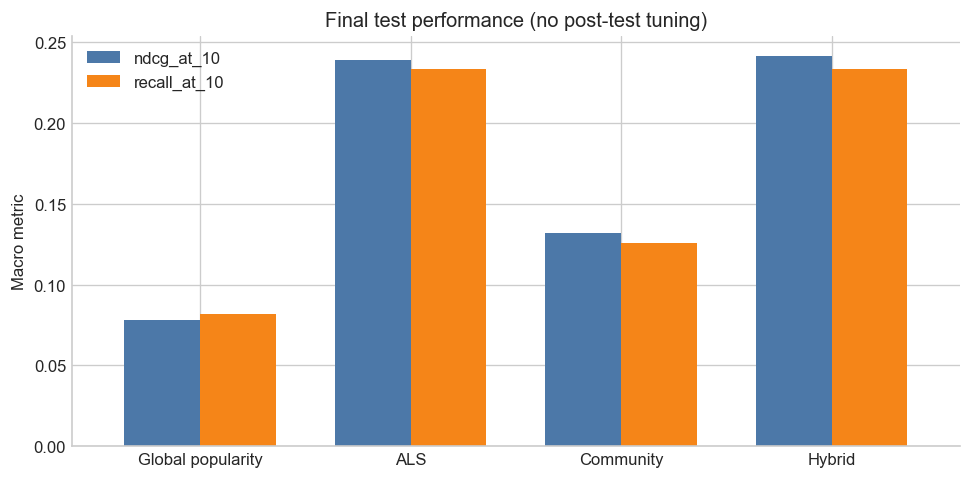
\includegraphics[width=0.86\textwidth]{report_assets/test_performance.png}
\caption{Final test macro metrics from the executed notebook. ALS and hybrid are close; the community-only model improves over global popularity but is substantially weaker than ALS. The test set was evaluated only after validation settings had been selected.}
\label{fig:performance}
\end{figure}

For \textbf{hybrid versus ALS recommendation performance}, the paired user-level mean difference was
\[
\overline{\metric{NDCG}_{\rm Hybrid}-\metric{NDCG}_{\rm ALS}}=0.0025794511.
\]
A 2,000-resample paired user bootstrap with seed 5101 gave the 95\% percentile interval
\[
[-0.0000075250,0.0050263518].
\]
The point estimate is positive, but the interval is not wholly above zero. The planned decision rule is therefore \emph{not met}; the study does not establish superiority or statistical significance. Recall@10 was marginally lower for the hybrid than ALS.

For \textbf{listening similarity within communities}, the analysis included 1,869 matched anchors: 10 in the 5--10, 5 in the 11--20, and 1,854 in the 21--50 training-activity stratum; none were in 51+. Deterministic sampling selected one same-community and one different-community peer per anchor within stratum. The mean within-minus-cross training-set Jaccard similarity was 0.02017763. The descriptive leave-one-user-out jackknife SE was 0.00206150, with normal interval $[0.01613708,$ $0.02421818]$. Peers could recur: 1,638 unique peers were used and the maximum reuse was nine rows. Consequently, rows are dependent and the uncertainty is descriptive, not population-level or causal.

The \textbf{sparse-history subgroup analysis} was non-estimable. All 1,876 evaluation-eligible users satisfied the planned sparse cutoff of 35, leaving zero non-sparse users and hence no subgroup interaction contrast. Redefining the cutoff after observing this would have changed the estimand, so no alternative subgroup was introduced.

\begin{figure}[h]
\centering
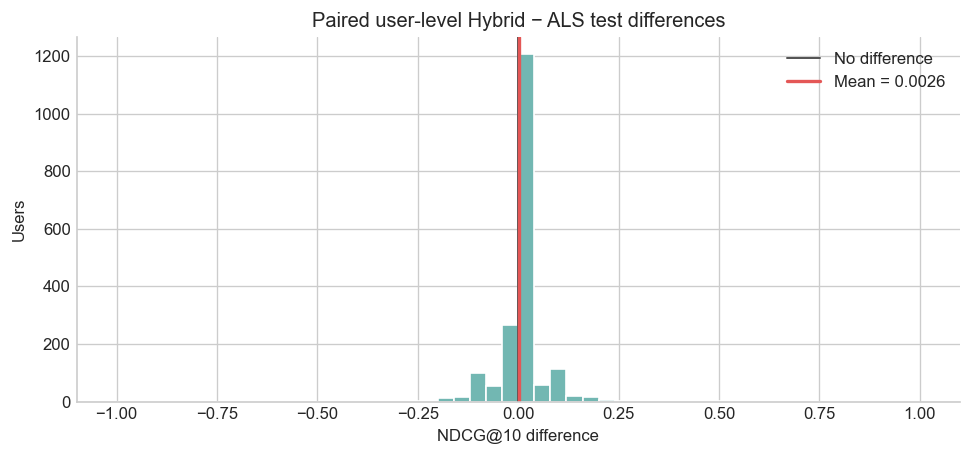
\includegraphics[width=0.78\textwidth]{report_assets/h2_differences.png}
\caption{Observed paired user-level Hybrid-minus-ALS NDCG@10 differences from the executed notebook. The red line is their mean, not a confidence bound. Most users have tied NDCG, while gains and losses occur on both sides; the inferential interval is reported in the text.}
\label{fig:paired-differences}
\end{figure}

\section{Insights and limitations}

The main pattern is complementarity without conclusive incremental accuracy. Community-only recommendation more than doubled global NDCG@10, and the positive listening-similarity contrast shows that same-community users had slightly more overlapping training artist sets under the matched descriptive design. Yet listening-based ALS captured most rank performance, and adding community scores produced only a 0.00258 NDCG point gain with an interval touching zero. The community signal appears real enough to aid a weak popularity model but too small, under this design, to demonstrate improvement over ALS.

The seeded shuffled-community diagnostic supports a structure-specific interpretation but is not a tuned comparison: shuffled community NDCG was 0.075667 versus 0.131956 with original labels, and shuffled hybrid NDCG was 0.235019 versus 0.241904. This decrease is consistent with useful alignment between the original communities and artist preferences, but a negative control cannot identify a causal social mechanism.

The full-catalog diagnostic expanded the universe from 16,057 to all 17,632 artists and made all 1,876 users metric-eligible. ALS NDCG fell to 0.226267 and hybrid NDCG to 0.228934 (global 0.074904; community 0.126024). The 1,575 fit-absent artists generated 2,954,700 cold-catalog candidates. ALS had the same number of missing item representations, community had the same number of valid zero probabilities, and the hybrid had the same number of missing components; all were placed after candidates with valid scores. This is a candidate-universe stress test, not learned new-item recommendation and not a tuning result.

Interpretation is limited by: (i) a small historical convenience sample; (ii) a static friendship topology that omits relationship timing and strength; (iii) no temporal listening information, so random-within-user holdout is not forecasting; (iv) source training histories capped at approximately 50 artists, producing many ties at the sparse cutoff and making the subgroup analysis non-estimable; (v) primary metrics conditional on retrievable relevance, excluding cold held-out items; (vi) a small, inconclusive hybrid improvement; and (vii) overlapping users and peers in the listening-similarity analysis. Aggregate counts are implicit signals, not ratings or dislikes. These limitations preclude causal interpretation and broad claims about cold-start users, new items, or present-day Last.fm behavior.

\section{Reproducibility information}

The executed \code{analysis.ipynb} is standalone: from the original archive it reconstructs validation, splitting, sparse labels, community membership, candidate sets, model selection, final refits, inference, and diagnostics in memory. It does not import local project modules or read cached analysis outputs. All code cells ran in order from a fresh Python 3.11 kernel, and the final run reproduced the reported values.

Dependencies are pinned in the submitted \code{requirements.txt}: implicit 0.7.2; NetworkX 3.2.1; NumPy 2.4.6; pandas 3.1.0; SciPy 1.17.1; Matplotlib 3.10.7; IPython kernel 7.1.0; nbclient 0.10.2; and nbformat 5.10.4. Execution used macOS arm64, seed 5101, and one numerical thread; the OpenBLAS, OMP, and MKL thread-count variables were each set to 1.

Reproduction requires the original \code{hetrec2011-lastfm-2k.zip}; the notebook reads it from \code{data/raw/}. Raw data are not redistributed. The notebook checks the expected data structure before analysis and reproduces the reported counts, selected configurations, and numeric results.

\section*{AI tool declaration}
\addcontentsline{toc}{section}{AI tool declaration}
I used ChatGPT to generate ideas, improve expression and report formatting, and review the clarity of the analysis and presentation. I am responsible for the content and quality of the submitted work.

\addcontentsline{toc}{section}{References}
\begin{thebibliography}{9}
\bibitem{cantador2011}
I. Cantador, P. Brusilovsky, and T. Kuflik.
Second Workshop on Information Heterogeneity and Fusion in Recommender Systems (HetRec 2011).
In \emph{Proceedings of the 5th ACM Conference on Recommender Systems}, pp. 387--388, 2011.
\href{https://doi.org/10.1145/2043932.2044016}{doi:10.1145/2043932.2044016}.

\bibitem{blondel2008}
V. D. Blondel, J.-L. Guillaume, R. Lambiotte, and E. Lefebvre.
Fast unfolding of communities in large networks.
\emph{Journal of Statistical Mechanics: Theory and Experiment}, 2008(10):P10008, 2008.
\href{https://doi.org/10.1088/1742-5468/2008/10/P10008}{doi:10.1088/1742-5468/2008/10/P10008}.

\bibitem{hu2008}
Y. Hu, Y. Koren, and C. Volinsky.
Collaborative filtering for implicit feedback datasets.
In \emph{Proceedings of the 8th IEEE International Conference on Data Mining}, pp. 263--272, 2008.
\href{https://doi.org/10.1109/ICDM.2008.22}{doi:10.1109/ICDM.2008.22}.

\bibitem{jarvelin2002}
K. J\"arvelin and J. Kek\"al\"ainen.
Cumulated gain-based evaluation of IR techniques.
\emph{ACM Transactions on Information Systems}, 20(4):422--446, 2002.
\href{https://doi.org/10.1145/582415.582418}{doi:10.1145/582415.582418}.

\end{thebibliography}

\end{document}
